\section{Pre-engagment}



\begin{figure}
  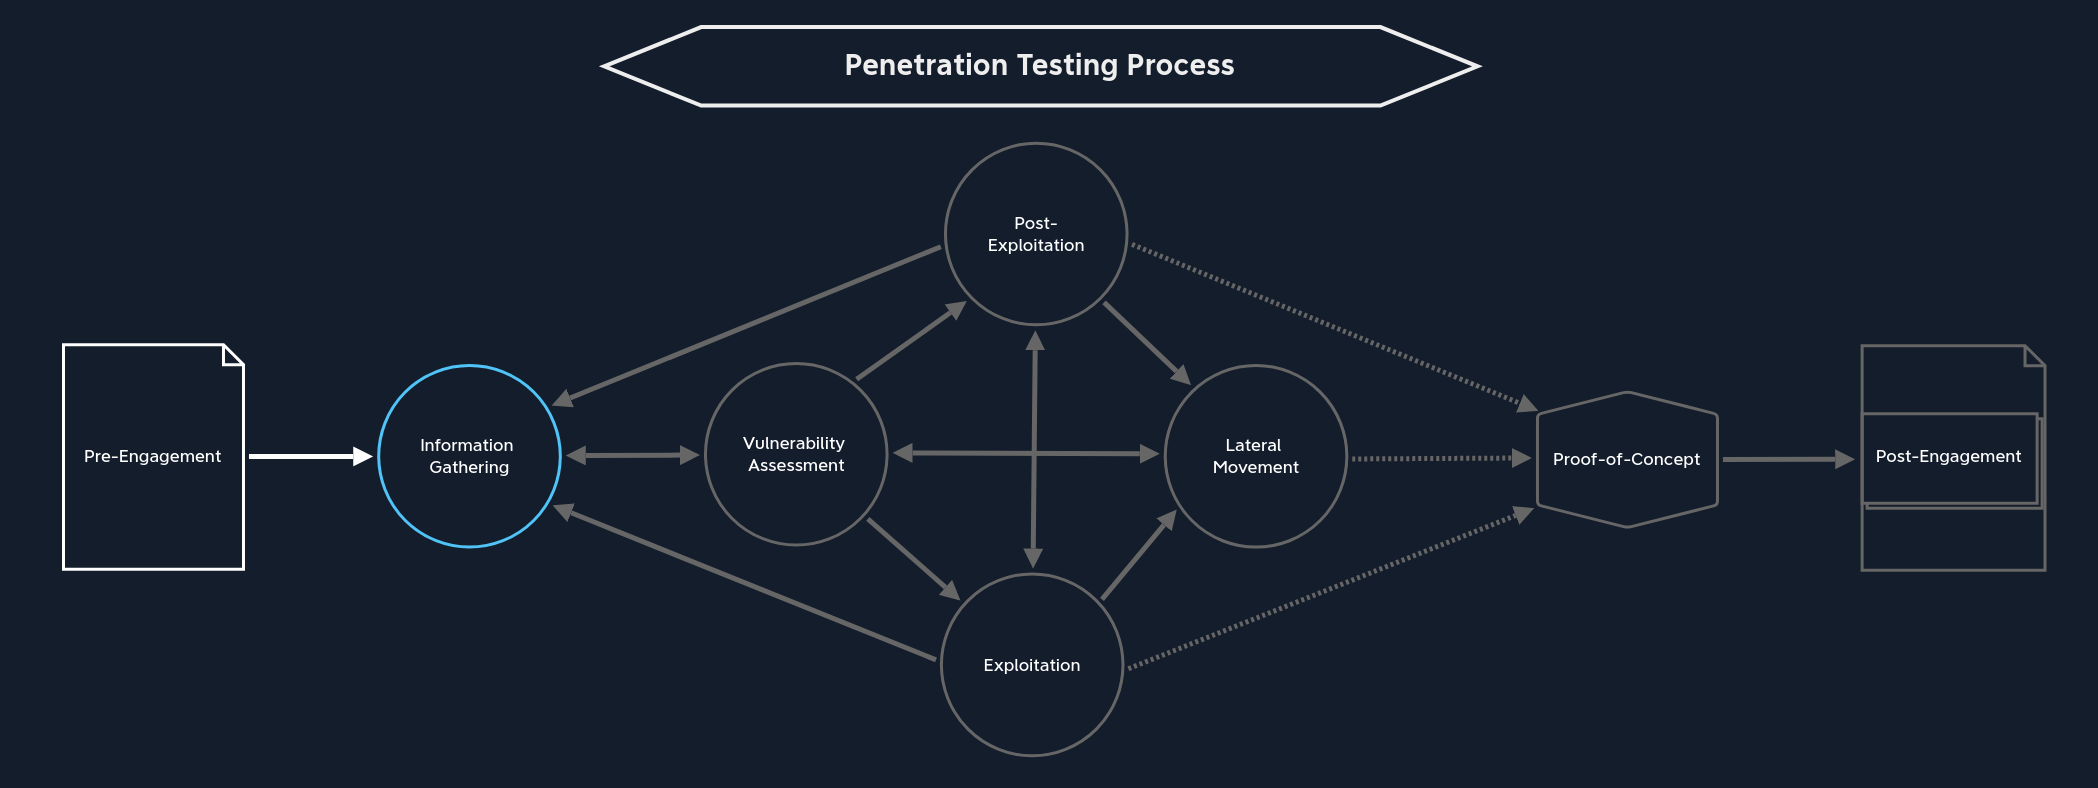
\includegraphics[width=\linewidth]{intro/process/images/pre.png}
  \caption{Pre-engagement}
  \label{fig:pentest-process-pre-engagement}
\end{figure}

The entire pre-engagement process consists of three essential components:
\begin{enumerate}
    \item Scoping questionnaire
    \item Pre-engagement meeting
    \item Kick-off meeting
\end{enumerate}

Before any of these can be discussed establish a NDA signed by all parties.
\begin{tabular}{ll}
Document &	Timing for Creation\\
Non-Disclosure Agreement (NDA) &	After Initial Contact \\
Scoping Questionnaire &	Before the Pre-Engagement Meeting \\
Scoping Document &	During the Pre-Engagement Meeting \\
Penetration Testing Proposal (Contract/Scope of Work (SoW)) &	During the
Pre-engagement Meeting\\
Rules of Engagement (RoE) &	Before the Kick-Off Meeting \\
Contractors Agreement (Physical Assessments) &	Before the Kick-Off Meeting \\
Reports &	During and after the conducted Penetration Test \\
\end{tabular}

\subsection{Scoping Questionnaire}

After initial contact is made with the client, we typically send them a Scoping Questionnaire to better understand the services they are seeking. This scoping questionnaire should clearly explain our services and may typically ask them to choose one or more from the following list:

\begin{tabular}{ll}
Internal Vulnerability Assessment &	 External Vulnerability Assessment\\
Internal Penetration Test &	 External Penetration Test\\
Wireless Security Assessment &	 Application Security Assessment\\
Physical Security Assessment &	 Social Engineering Assessment\\
Red Team Assessment &	 Web Application Security Assessment\\
\end{tabular}

nder each of these, the questionnaire should allow the client to be more
specific about the required assessment. Do they need a web application or
mobile application assessment? Secure code review? Should the Internal
Penetration Test be black box and semi-evasive? Do they want just a Phishing
assessment as part of the Social Engineering Assessment or also Vishing calls?
This is our chance to explain the depth and breadth of our services, ensure
that we understand our client's needs and expectations, and ensure that we can
adequately deliver the assessment they require.

Aside from the assessment type, client name, address, and key personnel contact information, some other critical pieces of information include:
\begin{itemize}
        \item How many expected live hosts?
        \item How many IPs/CIDR ranges in scope?
        \item How many Domains/Subdomains are in scope?
        \item How many wireless SSIDs in scope?
        \item How many web/mobile applications? If testing is authenticated, how many roles (standard user, admin, etc.)?
        \item For a Phishing assessment, how many users will be targeted? Will the client provide a list, or we will be required to gather this list via OSINT?
        \item If the client is requesting a Physical Assessment, how many locations? If multiple sites are in-scope, are they geographically dispersed?
        \item What is the objective of the Red Team Assessment? Are any activities (such as Phishing or physical security attacks) out of scope?
        \item Is a separate Active Directory Security Assessment desired?
        \item Will network testing be conducted from an anonymous user on the network or a standard domain user?
        \item Do we need to bypass Network Access Control (NAC)?
\end{itemize}

Finally, we will want to ask about information disclosure and evasiveness (if applicable to the assessment type):

\begin{itemize}
        \item Is the Penetration Test black box (no information provided), grey box (only IP address/CIDR ranges/URLs provided), white box (detailed information provided)

        \item Would they like us to test from a non-evasive, hybrid-evasive (start quiet and gradually become "louder" to assess at what level the client's security personnel detect our activities), or fully evasive.
\end{itemize}


\subsection{Pre-Engagement Meeting}
This meeting discusses all relevant and essential components with the customer before the penetration test, explaining them to our customer. The information we gather during this phase, along with the data collected from the scoping questionnaire, will serve as inputs to the Penetration Testing Proposal, also known as the Contract or Scope of Work (SoW).
\subsubsection{Contract checklist}
\begin{itemize}
\item {\emph NDA}
\item  Goals 	Goals are milestones that must be achieved during the order/project. In this process, goal setting is started with the significant goals and continued with fine-grained and small ones.
\item  {\emph Scope} 	The individual components to be tested are discussed and defined. These may include domains, IP ranges, individual hosts, specific accounts, security systems, etc. Our customers may expect us to find out one or the other point by ourselves. However, the legal basis for testing the individual components has the highest priority here.
\item  {\emph Penetration Testing Type} 	When choosing the type of penetration test, we present the individual options and explain the advantages and disadvantages. Since we already know the goals and scope of our customers, we can and should also make a recommendation on what we advise and justify our recommendation accordingly. Which type is used in the end is the client's decision.
\item  {\emph Methodologies} 	Examples: OSSTMM, OWASP, automated and manual unauthenticated analysis of the internal and external network components, vulnerability assessments of network components and web applications, vulnerability threat vectorization, verification and exploitation, and exploit development to facilitate evasion techniques.
\item  {\emph Penetration Testing Locations} 	External: Remote (via secure VPN) and/or Internal: Internal or Remote (via secure VPN)
\item  {\emph Time Estimation} 	For the time estimation, we need the start and the end date for the penetration test. This gives us a precise time window to perform the test and helps us plan our procedure. It is also vital to explicitly ask how time windows the individual attacks (Exploitation / Post-Exploitation / Lateral Movement) are to be carried out. These can be carried out during or outside regular working hours. When testing outside regular working hours, the focus is more on the security solutions and systems that should withstand our attacks.
\item  {\emph Third Parties} 	For the third parties, it must be determined via which third-party providers our customer obtains services. These can be cloud providers, ISPs, and other hosting providers. Our client must obtain written consent from these providers describing that they agree and are aware that certain parts of their service will be subject to a simulated hacking attack. It is also highly advisable to require the contractor to forward the third-party permission sent to us so that we have actual confirmation that this permission has indeed been obtained.
\item  {\emph Evasive Testing} 	Evasive testing is the test of evading and passing security traffic and security systems in the customer's infrastructure. We look for techniques that allow us to find out information about the internal components and attack them. It depends on whether our contractor wants us to use such techniques or not.
\item  {\emph Risks} 	We must also inform our client about the risks involved in the tests and the possible consequences. Based on the risks and their potential severity, we can then set the limitations together and take certain precautions.
\item  {\emph Scope Limitations  \& Restrictions} 	It is also essential to determine which servers, workstations, or other network components are essential for the client's proper functioning and its customers. We will have to avoid these and must not influence them any further, as this could lead to critical technical errors that could also affect our client's customers in production.
\item  {\emph Information Handling} 	HIPAA, PCI, HITRUST, FISMA/NIST, etc.
\item  {\emph Contact Information} 	For the contact information, we need to create a list of each person's name, title, job title, e-mail address, phone number, office phone number, and an escalation priority order.
\item  {\emph Lines of Communication} 	It should also be documented which communication channels are used to exchange information between the customer and us. This may involve e-mail correspondence, telephone calls, or personal meetings.
\item  {\emph Reporting} 	Apart from the report's structure, any customer-specific requirements the report should contain are also discussed. In addition, we clarify how the reporting is to take place and whether a presentation of the results is desired.
\item  {\emph Payment Terms} 	Finally, prices and the terms of payment are explained.
\end{itemize}

The most crucial element of this meeting is the detailed presentation of the
penetration test to our client and its focus. As we already know, each piece of
infrastructure is unique for the most part, and each client has particular
preferences on which they place the most importance. Finding out these
priorities is an essential part of this meeting.
\subsubsection{Rules of Engagement - Checklist}
\begin{itemize}
    \item {\emph Introduction} 	Description of this document.
    \item {\emph Contractor} 	Company name, contractor full name, job title.
    \item {\emph Penetration Testers} 	Company name, pentesters full name.
    \item {\emph Contact Information} 	Mailing addresses, e-mail addresses, and phone numbers of all client parties and penetration testers.
    \item {\emph Purpose} 	Description of the purpose for the conducted penetration test.
    \item {\emph Goals} 	Description of the goals that should be achieved with the penetration test.
    \item {\emph Scope} 	All IPs, domain names, URLs, or CIDR ranges.
    \item {\emph Lines of Communication} 	Online conferences or phone calls or face-to-face meetings, or via e-mail.
    \item {\emph Time Estimation} 	Start and end dates.
    \item {\emph Time of the Day to Test} 	Times of the day to test.
    \item {\emph Penetration Testing Type} 	External/Internal Penetration Test/Vulnerability Assessments/Social Engineering.
    \item {\emph Penetration Testing Locations} 	Description of how the connection to the client network is established.
    \item {\emph Methodologies} 	OSSTMM, PTES, OWASP, and others.
    \item {\emph Objectives / Flags} 	Users, specific files, specific information, and others.
    \item {\emph Evidence Handling} 	Encryption, secure protocols
    \item {\emph System Backups} 	Configuration files, databases, and others.
    \item {\emph Information Handling} 	Strong data encryption
    \item {\emph Incident Handling and Reporting} 	Cases for contact, pentest interruptions, type of reports
    \item {\emph Status Meetings} 	Frequency of meetings, dates, times, included parties
    \item {\emph Reporting} 	Type, target readers, focus
    \item {\emph Retesting} 	Start and end dates
    \item {\emph Disclaimers and Limitation of Liability} 	System damage, data loss
    \item {\emph Permission to Test} 	Signed contract, contractors agreement
\end{itemize}

\subsection{Kick-Off Meeting}

 We will go over the nature of the penetration test and how it will take place.
 Usually, there is no Denial of Service (DoS) testing. We also explain that if
 a critical vulnerability is identified, penetration testing activities will be
 paused, a vulnerability notification report will be generated, and the
 emergency contacts will be contacted. Typically these are only generated
 during External Penetration Tests for critical flaws such as unauthenticated
 remote code execution (RCE), SQL injection, or another flaw that leads to
 sensitive data disclosure. The purpose of this notification is to allow the
 client to assess the risk internally and determine if the issue warrants an
 emergency fix. We would typically only stop an Internal Penetration Test and
 alert the client if a system becomes unresponsive, we find evidence of illegal
 activity (such as illegal content on a file share) or the presence of an
 external threat actor in the network or a prior breach.

 xplaining the penetration testing process gives everyone involved a clear idea of our entire process. This demonstrates our professional approach and convinces our questioners that we know what we are doing. Because apart from the technical staff, CTO, and CISO, it will sound like a certain kind of magic that is very difficult for non-technical professionals to understand. So we must be mindful of our audience and target the most technically inexperienced questioner so our approach can be followed by everyone we talk to.

All points related to testing need to be discussed and clarified. It is crucial to respond precisely to the wishes and expectations of the customer/client. Every company structure and network is different and requires an adapted approach. Each client has different goals, and we should adjust our testing to their wishes. We can typically see how experienced our clients are in undergoing penetration tests early in the call, so we may have to shift our focus to explain things in more detail and be prepared to field more questions, or the kickoff call may be very quick and straightforward.

\subsection{Contractors Agreement}
f the penetration test also includes physical testing, then an additional
contractor's agreement is required. Since it is not only a virtual environment
but also a physical intrusion, completely different laws apply here. It is also
possible that many of the employees have not been informed about the test.
Suppose we encounter employees with a very high-security awareness during the
physical attack and social engineering attempts, and we get caught. In that
case, the employees will, in most cases, contact the police. This additional
contractor's agreement is our "get out of jail free card" in this case. 

Checkpoint:
\begin{itemize}
\item Introduction
\item Contractor
\item Purpose
\item Goal
\item Penetration Testers
\item Contact Information
\item Physical Addresses
\item Building Name
\item Floors
\item Physical Room Identifications
\item Physical Components
\item Timeline
\item Notarization
\item Permission to Test
\end{itemize}
